\documentclass{standalone}
\usepackage{tikz}
\usetikzlibrary{patterns, positioning}
\usepackage[sfdefault]{ClearSans} %% option 'sfdefault' activates Clear Sans as the default text font
\usepackage[T1]{fontenc}

\begin{document}
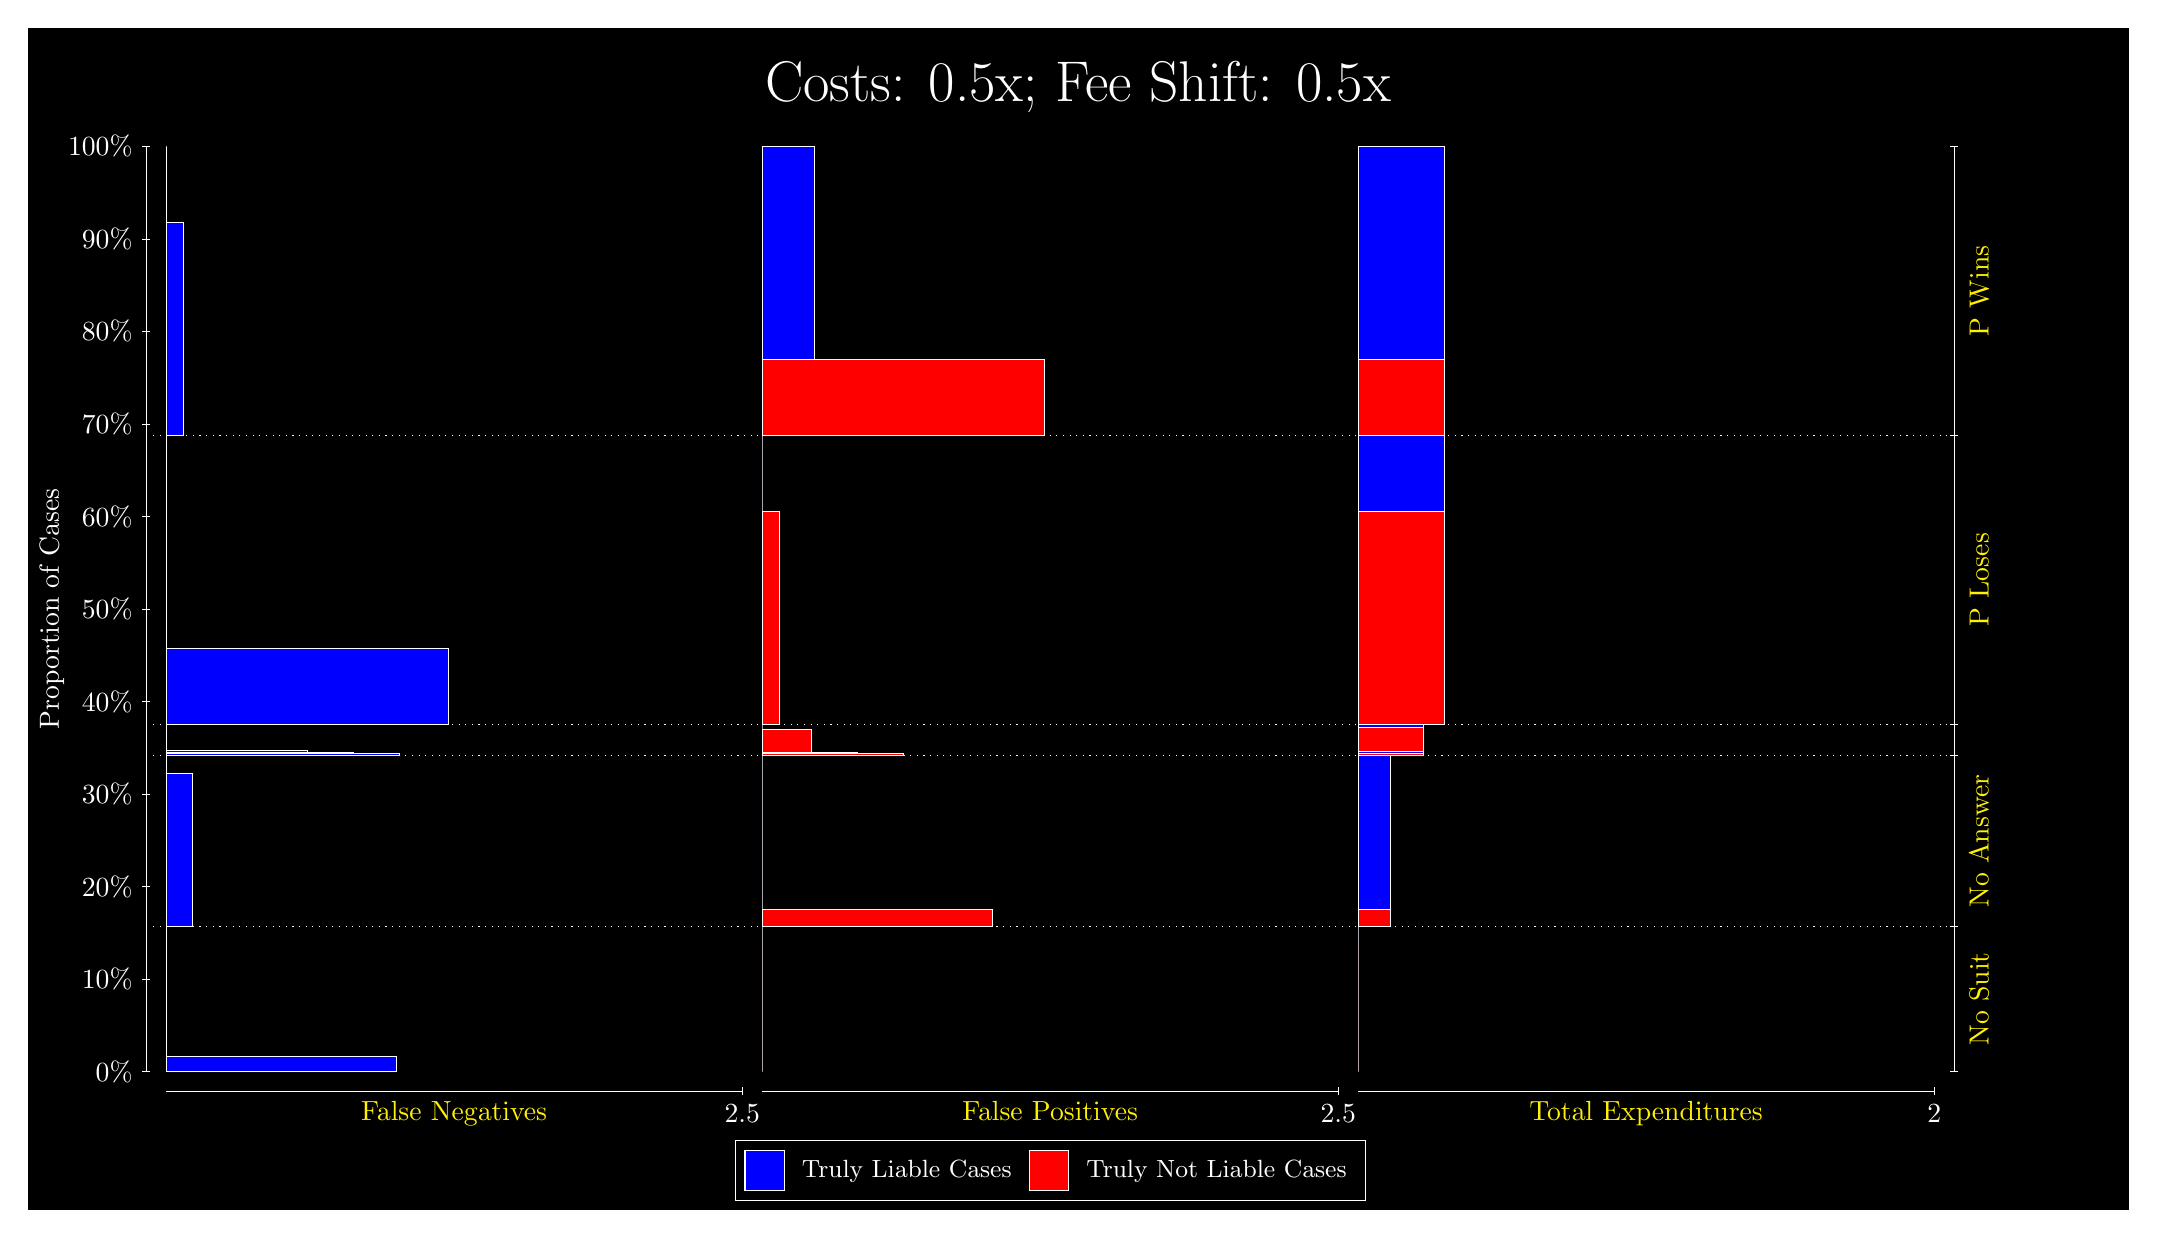
\begin{tikzpicture}
\draw[fill=black] (0,0) rectangle (26.667,15);
\draw[text=white] (0,13.5) rectangle (26.667,15) node[midway] {\huge Costs: 0.5x; Fee Shift: 0.5x};
\draw[white, very thin] (1.5,1.75) -- (1.5,13.5);
\node[rotate=90, text=white, anchor=center] at (0.3, 7.625) {Proportion of Cases};
\draw[white, very thin] (1.45,1.75) -- (1.55,1.75);
\node[text=white, anchor=east] at (1.45, 1.75) {0\%};
\draw[white, very thin] (1.45,2.925) -- (1.55,2.925);
\node[text=white, anchor=east] at (1.45, 2.925) {10\%};
\draw[white, very thin] (1.45,4.1) -- (1.55,4.1);
\node[text=white, anchor=east] at (1.45, 4.1) {20\%};
\draw[white, very thin] (1.45,5.275) -- (1.55,5.275);
\node[text=white, anchor=east] at (1.45, 5.275) {30\%};
\draw[white, very thin] (1.45,6.45) -- (1.55,6.45);
\node[text=white, anchor=east] at (1.45, 6.45) {40\%};
\draw[white, very thin] (1.45,7.625) -- (1.55,7.625);
\node[text=white, anchor=east] at (1.45, 7.625) {50\%};
\draw[white, very thin] (1.45,8.8) -- (1.55,8.8);
\node[text=white, anchor=east] at (1.45, 8.8) {60\%};
\draw[white, very thin] (1.45,9.975) -- (1.55,9.975);
\node[text=white, anchor=east] at (1.45, 9.975) {70\%};
\draw[white, very thin] (1.45,11.15) -- (1.55,11.15);
\node[text=white, anchor=east] at (1.45, 11.15) {80\%};
\draw[white, very thin] (1.45,12.325) -- (1.55,12.325);
\node[text=white, anchor=east] at (1.45, 12.325) {90\%};
\draw[white, very thin] (1.45,13.5) -- (1.55,13.5);
\node[text=white, anchor=east] at (1.45, 13.5) {100\%};

\draw[white, very thin] (24.457,1.75) -- (24.457,13.5);
\draw[white, very thin] (24.407,1.75) -- (24.507,1.75);
\node[anchor=west] at (24.407, 1.75) {};
\draw[white, very thin] (24.407,3.5919) -- (24.507,3.5919);
\node[anchor=west] at (24.407, 3.5919) {};
\draw[white, very thin] (24.407,5.7647) -- (24.507,5.7647);
\node[anchor=west] at (24.407, 5.7647) {};
\draw[white, very thin] (24.407,6.1618) -- (24.507,6.1618);
\node[anchor=west] at (24.407, 6.1618) {};
\draw[white, very thin] (24.407,9.8309) -- (24.507,9.8309);
\node[anchor=west] at (24.407, 9.8309) {};
\draw[white, very thin] (24.407,13.5) -- (24.507,13.5);
\node[anchor=west] at (24.407, 13.5) {};

\draw[white, very thin, fill=blue] (1.75,1.75) rectangle (4.6775,1.9438);
\draw[white, very thin, fill=red] (1.75,1.9438) rectangle (1.75,3.5919);
\draw[white, very thin, fill=blue] (1.75,3.5919) rectangle (2.0793,5.5414);
\draw[white, very thin, fill=red] (1.75,5.5414) rectangle (1.75,5.7647);
\draw[white, very thin, fill=blue] (1.75,5.7647) rectangle (4.7141,5.7965);
\draw[white, very thin, fill=blue] (1.75,5.7965) rectangle (4.1286,5.7997);
\draw[white, very thin, fill=blue] (1.75,5.7997) rectangle (3.5431,5.8273);
\draw[white, very thin, fill=red] (1.75,5.8273) rectangle (1.75,6.1618);
\draw[white, very thin, fill=blue] (1.75,6.1618) rectangle (5.3362,7.1315);
\draw[white, very thin, fill=red] (1.75,7.1315) rectangle (1.75,9.8309);
\draw[white, very thin, fill=blue] (1.75,9.8309) rectangle (1.9696,12.53);
\draw[white, very thin, fill=red] (1.75,12.53) rectangle (1.75,13.5);
\draw[white, very thin, fill=red] (9.3189,1.75) rectangle (9.3189,3.3981);
\draw[white, very thin, fill=blue] (9.3189,3.3981) rectangle (9.3189,3.5919);
\draw[white, very thin, fill=red] (9.3189,3.5919) rectangle (12.246,3.8152);
\draw[white, very thin, fill=blue] (9.3189,3.8152) rectangle (9.3189,5.7647);
\draw[white, very thin, fill=red] (9.3189,5.7647) rectangle (11.112,5.7923);
\draw[white, very thin, fill=red] (9.3189,5.7923) rectangle (10.526,5.7994);
\draw[white, very thin, fill=red] (9.3189,5.7994) rectangle (9.941,6.0993);
\draw[white, very thin, fill=blue] (9.3189,6.0993) rectangle (9.3189,6.1618);
\draw[white, very thin, fill=red] (9.3189,6.1618) rectangle (9.5384,8.8612);
\draw[white, very thin, fill=blue] (9.3189,8.8612) rectangle (9.3189,9.8309);
\draw[white, very thin, fill=red] (9.3189,9.8309) rectangle (12.905,10.801);
\draw[white, very thin, fill=blue] (9.3189,10.801) rectangle (9.9776,13.5);
\draw[white, very thin, fill=red] (16.888,1.75) rectangle (16.888,3.3981);
\draw[white, very thin, fill=blue] (16.888,3.3981) rectangle (16.888,3.5919);
\draw[white, very thin, fill=red] (16.888,3.5919) rectangle (17.299,3.8152);
\draw[white, very thin, fill=blue] (16.888,3.8152) rectangle (17.299,5.7647);
\draw[white, very thin, fill=red] (16.888,5.7647) rectangle (17.711,5.7923);
\draw[white, very thin, fill=blue] (16.888,5.7923) rectangle (17.711,5.8199);
\draw[white, very thin, fill=red] (16.888,5.8199) rectangle (17.711,6.1268);
\draw[white, very thin, fill=blue] (16.888,6.1268) rectangle (17.711,6.1618);
\draw[white, very thin, fill=red] (16.888,6.1618) rectangle (17.986,8.8612);
\draw[white, very thin, fill=blue] (16.888,8.8612) rectangle (17.986,9.8309);
\draw[white, very thin, fill=red] (16.888,9.8309) rectangle (17.986,10.801);
\draw[white, very thin, fill=blue] (16.888,10.801) rectangle (17.986,13.5);
\draw[white, dotted] (1.5,3.5919) -- (24.457,3.5919);
\draw[white, dotted] (1.5,5.7647) -- (24.457,5.7647);
\draw[white, dotted] (1.5,6.1618) -- (24.457,6.1618);
\draw[white, dotted] (1.5,9.8309) -- (24.457,9.8309);
\draw[white, very thin] (1.75,1.5) -- (9.0689,1.5);
\node[text=yellow, anchor=north] at (5.4094, 1.5) {False Negatives};
\draw[white, very thin] (9.0689,1.45) -- (9.0689,1.55);
\node[text=white, anchor=north] at (9.0689, 1.45) {2.5};

\draw[white, very thin] (9.3189,1.5) -- (16.638,1.5);
\node[text=yellow, anchor=north] at (12.978, 1.5) {False Positives};
\draw[white, very thin] (16.638,1.45) -- (16.638,1.55);
\node[text=white, anchor=north] at (16.638, 1.45) {2.5};

\draw[white, very thin] (16.888,1.5) -- (24.207,1.5);
\node[text=yellow, anchor=north] at (20.547, 1.5) {Total Expenditures};
\draw[white, very thin] (24.207,1.45) -- (24.207,1.55);
\node[text=white, anchor=north] at (24.207, 1.45) {2};

\node[text=yellow, centered, rotate=90] at (24.777, 2.6709) {No Suit};
\node[text=yellow, centered, rotate=90] at (24.777, 4.6783) {No Answer};

\node[text=yellow, centered, rotate=90] at (24.777, 7.9964) {P Loses};
\node[text=yellow, centered, rotate=90] at (24.777, 11.665) {P Wins};

\draw (12.978300999999998,1.5) node[draw=none] (baseCoordinate) {};
\begin{scope}[align=center]
        \matrix[scale=0.5, draw=white, below=0.5cm of baseCoordinate, nodes={draw}, column sep=0.1cm]{
            \node[rectangle, draw, minimum width=0.5cm, minimum height=0.5cm, fill=blue] {}; &
            \node[draw=none, font=\small, text=white] (B) {Truly Liable Cases}; &
            \node[rectangle, draw, minimum width=0.5cm, minimum height=0.5cm, fill=red] {}; &
            \node[draw=none, font=\small, text=white] (B) {Truly Not Liable Cases}; \\
            };
\end{scope}

\end{tikzpicture}
\end{document}